\section{Introduction}

The Kalman Filter operates based on the state space representation provided:
\[\begin{cases}
    \mathbf{x}(t+1)=\mathbf{Fx}(t)+\mathbf{Gu}(t)+\mathbf{v}_1(t) \\
    \mathbf{y}(t)=\mathbf{Hx}(t)+\mathbf{Du}(t)+\mathbf{v}_2(t)
\end{cases}\]
In this representation, two distinct noises are considered: $v_1(t)$ and $v_2(t)$. 
It's important to note that this model is typically provided in a white-box method, where the system dynamics are known or assumed.

\paragraph*{Kalman Filter usage}
Given a dataset:
\[\left\{ u(1),u(2),\dots,u(N)\right\},\left\{ y(1),y(2),\dots,y(N)\right\}\]
Where the current time is $N$, we can address the following tasks:
\begin{enumerate}
    \item \textit{Predicting output $k$ steps ahead}. 
        The objective is to forecast the output at $k$ steps ahead:
        \[\hat{y}(N+k\mid N)\]
        This task can also be tackled using ARMAX models, resulting in the same prediction.
    \item \textit{Predicting state $k$ steps ahead}.
        The aim is to estimate the state at $k$ steps ahead:
        \[\hat{\mathbf{x}}(N+k\mid N)\]
        Unlike ARMAX models, which can only predict the output, this problem cannot be resolved using them.
    \item \textit{Filtering the present state}. 
        The goal is to determine the state at the current time $N$:
        \[\hat{\mathbf{x}}(N\mid N)\]
        This constitutes a filtering challenge rather than a predictive one. 
        ARMAX models are incapable of solving this.
    \item \textit{Gray-box system identification}: although not the primary focus of the Kalman Filter, it can provide auxiliary benefits in system identification.
\end{enumerate}

\subsection{Software sensing}
Consider a generic system with $u(t)$ as inputs (actuators or control variables) and $y(t)$ as outputs (sensors, measurable variables). 
The system also contains internal states $x(t)$.
\begin{figure}[H]
    \centering
    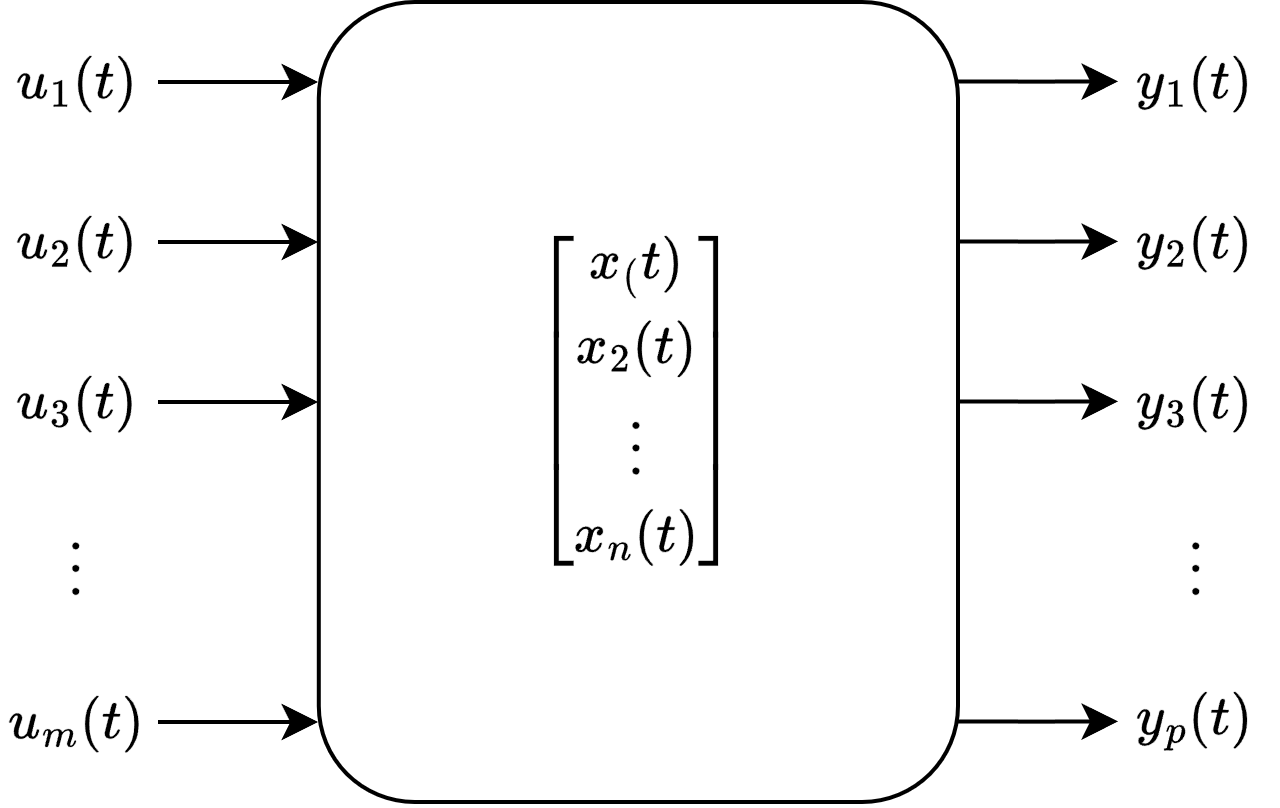
\includegraphics[width=0.4\linewidth]{images/mimo.png}
    \caption{Generic multiple input multiple output system}
\end{figure}
The depicted system is multiple input multiple output with $m$ inputs, $p$ outputs, and $n$ states.
Typically, the number of states is much greater than the number of outputs ($n \gg p$).
This is due to sensor cost considerations and the need to minimize their number.

Not all states are usually measured, but having the full state vector available is valuable for:
\begin{itemize}
    \item Designing control algorithms.
    \item Monitoring the system, including fault detection and predictive maintenance.
\end{itemize}
This problem can be addressed by adding physical sensors or by developing software sensing algorithms.
\begin{figure}[H]
    \centering
    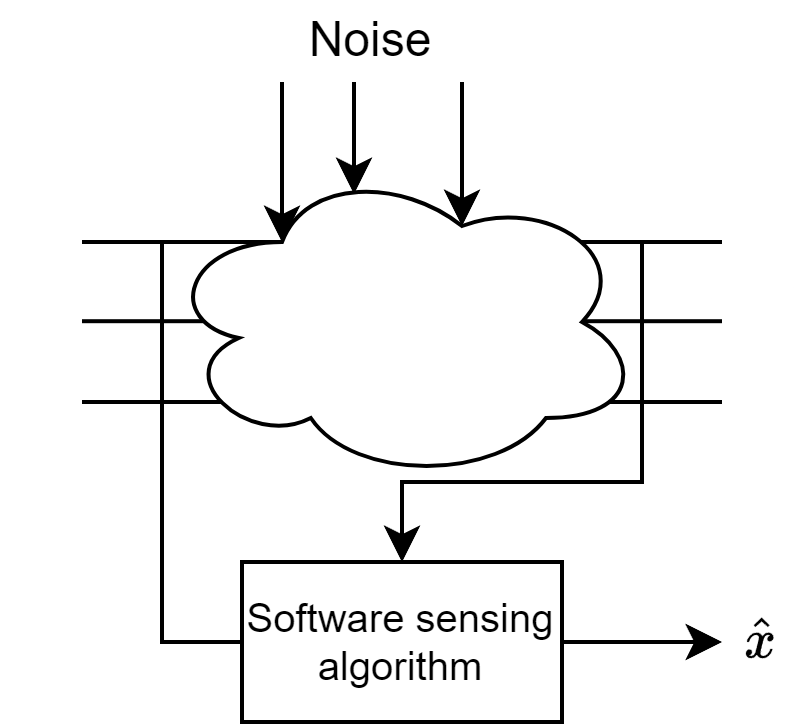
\includegraphics[width=0.4\linewidth]{images/sws.png}
    \caption{Software sensing}
\end{figure}
The software for estimation typically runs on another device with appropriate configuration.

\paragraph*{Issues with software sensing}
One must verify the observability of full states from the outputs to ascertain the feasibility of software sensing. 
If feasible, it's crucial to assess the level of noise in the estimation. 
The estimation error is deemed acceptable if it's comparable to sensor noise.

\subsection{Software sensing application}
Designers often face the decision between physical and software sensing. 
When physical sensing is not an option, software sensing becomes the only viable choice. 
However, when both options are available, a balance must be struck between development and hardware costs.

The development cost remains fixed, while the sensor cost varies based on the number of sensors required:
\begin{itemize}
    \item For small-volume applications, installing physical sensors may be more cost-effective.
    \item Conversely, for high-volume applications, software sensing tends to be the more economical choice.
\end{itemize}
In some instances, both methods may be employed for redundancy, particularly in safety-critical applications.